\documentclass{article}\usepackage[]{graphicx}\usepackage[]{xcolor}
% maxwidth is the original width if it is less than linewidth
% otherwise use linewidth (to make sure the graphics do not exceed the margin)
\makeatletter
\def\maxwidth{ %
  \ifdim\Gin@nat@width>\linewidth
    \linewidth
  \else
    \Gin@nat@width
  \fi
}
\makeatother

\definecolor{fgcolor}{rgb}{0.345, 0.345, 0.345}
\newcommand{\hlnum}[1]{\textcolor[rgb]{0.686,0.059,0.569}{#1}}%
\newcommand{\hlsng}[1]{\textcolor[rgb]{0.192,0.494,0.8}{#1}}%
\newcommand{\hlcom}[1]{\textcolor[rgb]{0.678,0.584,0.686}{\textit{#1}}}%
\newcommand{\hlopt}[1]{\textcolor[rgb]{0,0,0}{#1}}%
\newcommand{\hldef}[1]{\textcolor[rgb]{0.345,0.345,0.345}{#1}}%
\newcommand{\hlkwa}[1]{\textcolor[rgb]{0.161,0.373,0.58}{\textbf{#1}}}%
\newcommand{\hlkwb}[1]{\textcolor[rgb]{0.69,0.353,0.396}{#1}}%
\newcommand{\hlkwc}[1]{\textcolor[rgb]{0.333,0.667,0.333}{#1}}%
\newcommand{\hlkwd}[1]{\textcolor[rgb]{0.737,0.353,0.396}{\textbf{#1}}}%
\let\hlipl\hlkwb

\usepackage{framed}
\makeatletter
\newenvironment{kframe}{%
 \def\at@end@of@kframe{}%
 \ifinner\ifhmode%
  \def\at@end@of@kframe{\end{minipage}}%
  \begin{minipage}{\columnwidth}%
 \fi\fi%
 \def\FrameCommand##1{\hskip\@totalleftmargin \hskip-\fboxsep
 \colorbox{shadecolor}{##1}\hskip-\fboxsep
     % There is no \\@totalrightmargin, so:
     \hskip-\linewidth \hskip-\@totalleftmargin \hskip\columnwidth}%
 \MakeFramed {\advance\hsize-\width
   \@totalleftmargin\z@ \linewidth\hsize
   \@setminipage}}%
 {\par\unskip\endMakeFramed%
 \at@end@of@kframe}
\makeatother

\definecolor{shadecolor}{rgb}{.97, .97, .97}
\definecolor{messagecolor}{rgb}{0, 0, 0}
\definecolor{warningcolor}{rgb}{1, 0, 1}
\definecolor{errorcolor}{rgb}{1, 0, 0}
\newenvironment{knitrout}{}{} % an empty environment to be redefined in TeX

\usepackage{alltt}
\IfFileExists{upquote.sty}{\usepackage{upquote}}{}
\begin{document}

\subsection{The package a4adiags}

The package `a4adiags` contains some additional diagnostics based on the \textcolor{red}{reference}.Runs test checks weather the residuals are randomly distributed. A "run" is a sequence of the same sign residuals. Few runs indicate a trend or a correlation in the residuals while too many runs may suggest overfitting. 
  The primary output of a runstest is a p-value where:
    - A high p value $(p\leq 0.05)$ suggests that the residuals are randomly distributed
    - A low p value indicates a non-random pattern in the residuals

\begin{knitrout}
\definecolor{shadecolor}{rgb}{0.969, 0.969, 0.969}\color{fgcolor}\begin{kframe}
\begin{alltt}
\hlkwd{library}\hldef{(FLa4a)}
\end{alltt}


{\ttfamily\noindent\itshape\color{messagecolor}{\#\# Loading required package: FLCore}}

{\ttfamily\noindent\itshape\color{messagecolor}{\#\# Loading required package: lattice}}

{\ttfamily\noindent\itshape\color{messagecolor}{\#\# Loading required package: iterators}}

{\ttfamily\noindent\itshape\color{messagecolor}{\#\# FLCore (Version 2.6.20.9201, packaged: 2024-07-08 21:29:30 UTC)}}

{\ttfamily\noindent\itshape\color{messagecolor}{\#\# Loading required package: triangle}}

{\ttfamily\noindent\itshape\color{messagecolor}{\#\# This is FLa4a 1.9.0. For overview type 'help(package="{}FLa4a"{})'}}\begin{alltt}
\hlkwd{library}\hldef{(FLCore)}
\hlkwd{library}\hldef{(a4adiags)}
\end{alltt}


{\ttfamily\noindent\itshape\color{messagecolor}{\#\# Loading required package: ggplot2}}

{\ttfamily\noindent\itshape\color{messagecolor}{\#\# \\\#\# Attaching package: 'ggplot2'}}

{\ttfamily\noindent\itshape\color{messagecolor}{\#\# The following object is masked from 'package:FLCore':\\\#\# \\\#\# \ \ \ \ \%+\%}}

{\ttfamily\noindent\itshape\color{messagecolor}{\#\# Loading required package: ggplotFL}}\begin{alltt}
\hlkwd{library}\hldef{(ggplot2);}\hlkwd{theme_set}\hldef{(}\hlkwd{theme_bw}\hldef{())}
\hlkwd{rm}\hldef{(}\hlkwc{list} \hldef{=} \hlkwd{ls}\hldef{())}
\hldef{fit05} \hlkwb{<-} \hlkwd{sca}\hldef{(mut09, mut09.idx,} \hlkwc{fmod} \hldef{=} \hlopt{~}\hlkwd{factor}\hldef{(age)} \hlopt{+} \hlkwd{s}\hldef{(year,} \hlkwc{k} \hldef{=} \hlnum{8}\hldef{))}
\hldef{res05} \hlkwb{<-} \hlkwd{residuals}\hldef{(fit05, mut09, mut09.idx)}
\end{alltt}
\end{kframe}
\end{knitrout}

\begin{knitrout}
\definecolor{shadecolor}{rgb}{0.969, 0.969, 0.969}\color{fgcolor}\begin{kframe}
\begin{alltt}
\hlkwd{plotRunstest}\hldef{(fit05, mut09.idx,} \hlkwc{combine} \hldef{= F)} \hlopt{+} \hlkwd{theme_bw}\hldef{()} \hlopt{+} \hlkwd{facet_wrap}\hldef{(}\hlopt{~}\hldef{age)}
\end{alltt}
\end{kframe}\begin{figure}
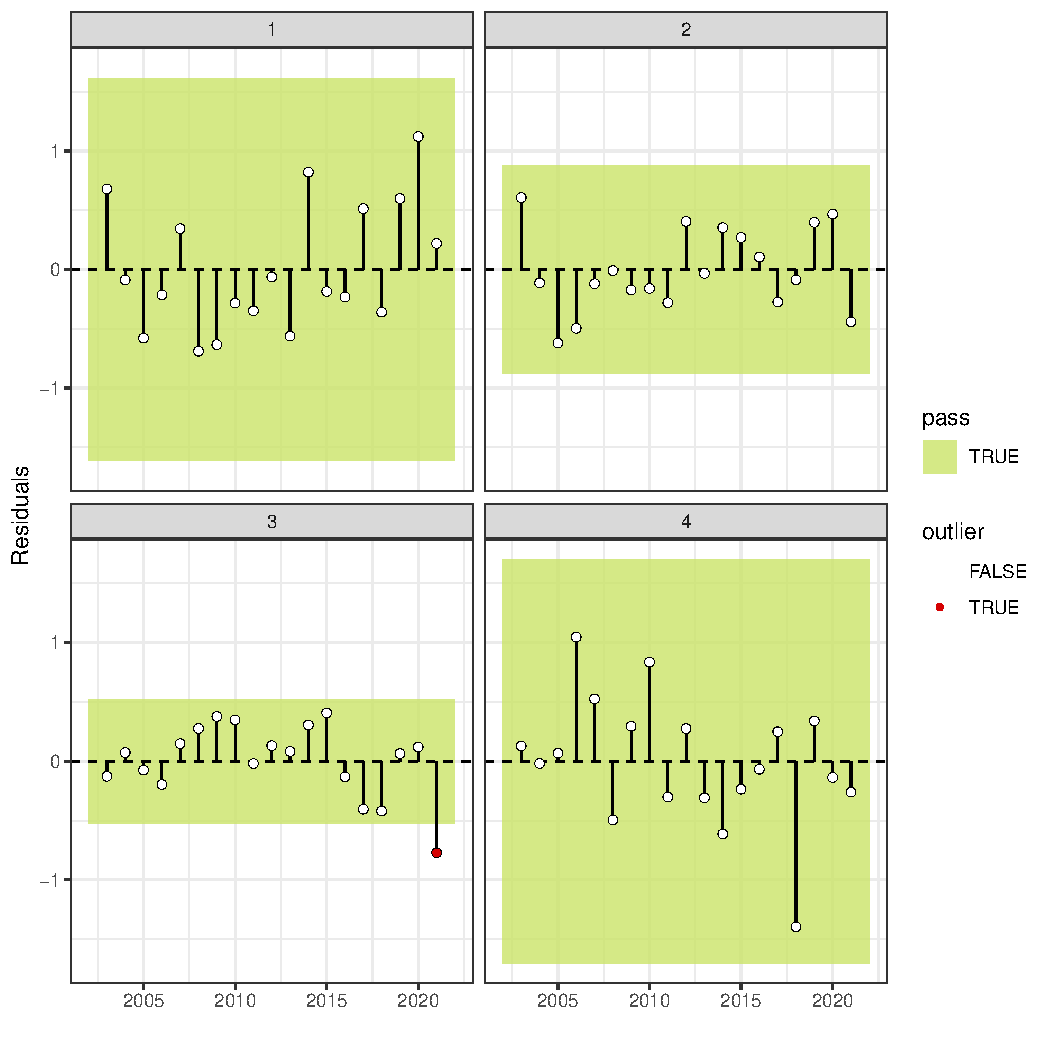
\includegraphics[width=\maxwidth]{figure/idxrunstest-1} \caption[Runstest for the index]{Runstest for the index}\label{fig:idxrunstest}
\end{figure}

\end{knitrout}

\begin{knitrout}
\definecolor{shadecolor}{rgb}{0.969, 0.969, 0.969}\color{fgcolor}\begin{kframe}
\begin{alltt}
\hlkwd{plotRunstest}\hldef{(}\hlkwd{catch.n}\hldef{(mut09),} \hlkwd{catch.n}\hldef{(mut09} \hlopt{+} \hldef{fit05),} \hlkwc{combine} \hldef{= F)} \hlopt{+} \hlkwd{theme_bw}\hldef{()} \hlopt{+} \hlkwd{facet_wrap}\hldef{(}\hlopt{~}\hldef{age)}
\end{alltt}
\end{kframe}\begin{figure}
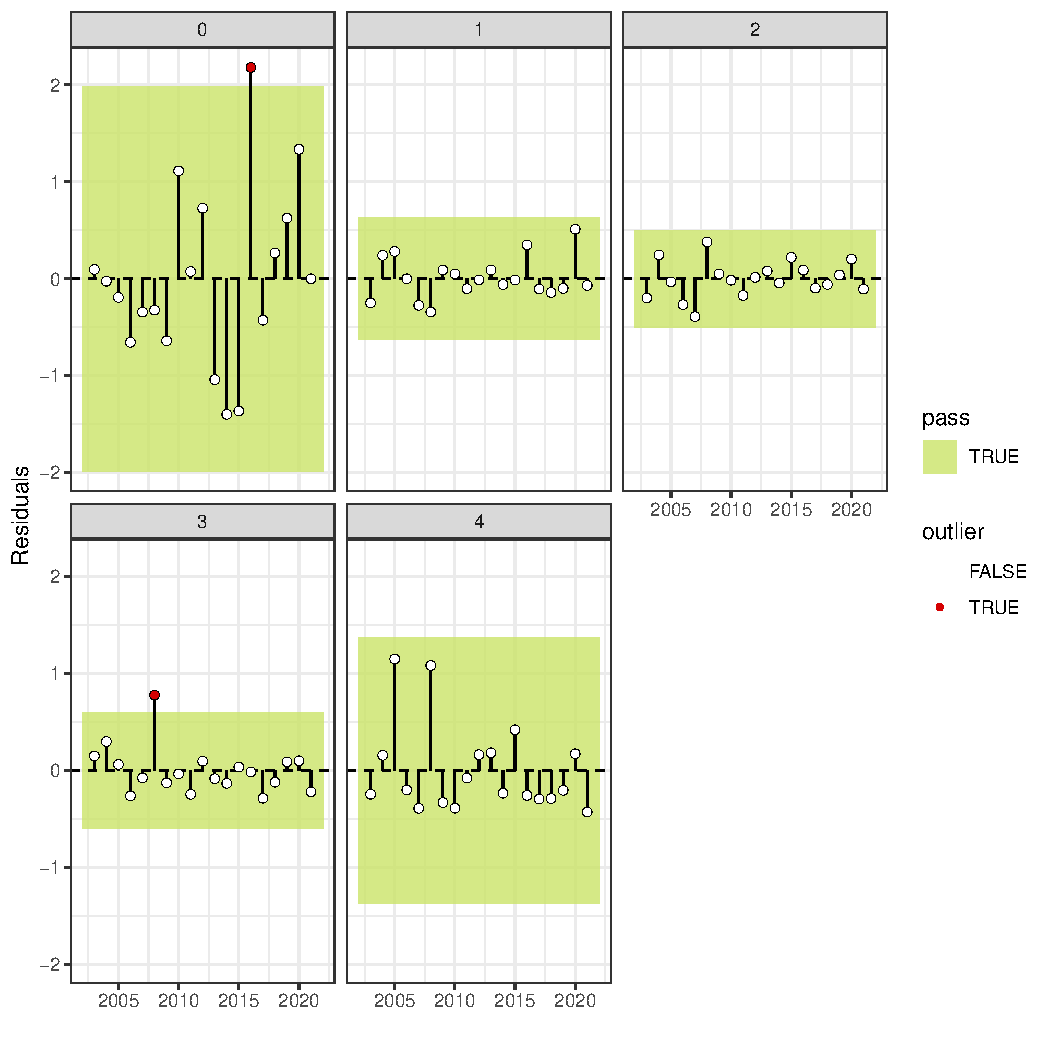
\includegraphics[width=\maxwidth]{figure/catchrunstest-1} \caption[Runstest for the catch]{Runstest for the catch}\label{fig:catchrunstest}
\end{figure}

\end{knitrout}

Green shading indicates no evidence $(p <  0.05)$ and red shading evidence $(p  >0.05)$ to reject the hypothesis of a randomly distributed time-series of residuals, respectively. The shaded (green/red) area spans three residual standard deviations to either side from zero, and the red points outside of the shading violate the ‘ $3\sigma$ limit’ for that series.

Hindcast is used to assess the prediction skill of the model by removing a couple of years from the end of the time series and forecasting for that years, to assess how close the projected values are to the ones assessed by the model. The hindcast can estimate forecast bias by comparing the forecasted values to the reference model estimates. The `a4adiags` package use a different approach, it is based on a technique proposed by Kell \textcolor{red}{ref} named hindcast cross-validation where the forecasted values are compared with the observed ones. Additionally mean absolute squared error is computed, a statistic for evaluating the prediction skill. MASE basically compares the model prediction skill against a random walk, i.e against the predicted value of a random process based only on the previous year's observation.

\begin{knitrout}
\definecolor{shadecolor}{rgb}{0.969, 0.969, 0.969}\color{fgcolor}\begin{kframe}
\begin{alltt}
\hldef{xval} \hlkwb{<-} \hlkwd{a4ahcxval}\hldef{(mut09,} \hlkwd{FLIndices}\hldef{(mut09.idx),} \hlkwc{nyears} \hldef{=} \hlnum{5}\hldef{,} \hlkwc{nsq} \hldef{=} \hlnum{3}\hldef{,} \hlkwc{fmodel} \hldef{=}  \hlopt{~}\hlkwd{factor}\hldef{(age)} \hlopt{+} \hlkwd{s}\hldef{(year,} \hlkwc{k} \hldef{=} \hlnum{8}\hldef{))}
\end{alltt}


{\ttfamily\noindent\color{warningcolor}{\#\# Warning: executing \%dopar\% sequentially: no parallel backend registered}}\begin{alltt}
\hlkwd{plotXval2}\hldef{(xval}\hlopt{$}\hldef{indices)} \hlopt{+} \hlkwd{ggtitle}\hldef{(}\hlkwd{paste0}\hldef{(}\hlsng{"Hindcast"}\hldef{))}
\end{alltt}
\end{kframe}\begin{figure}
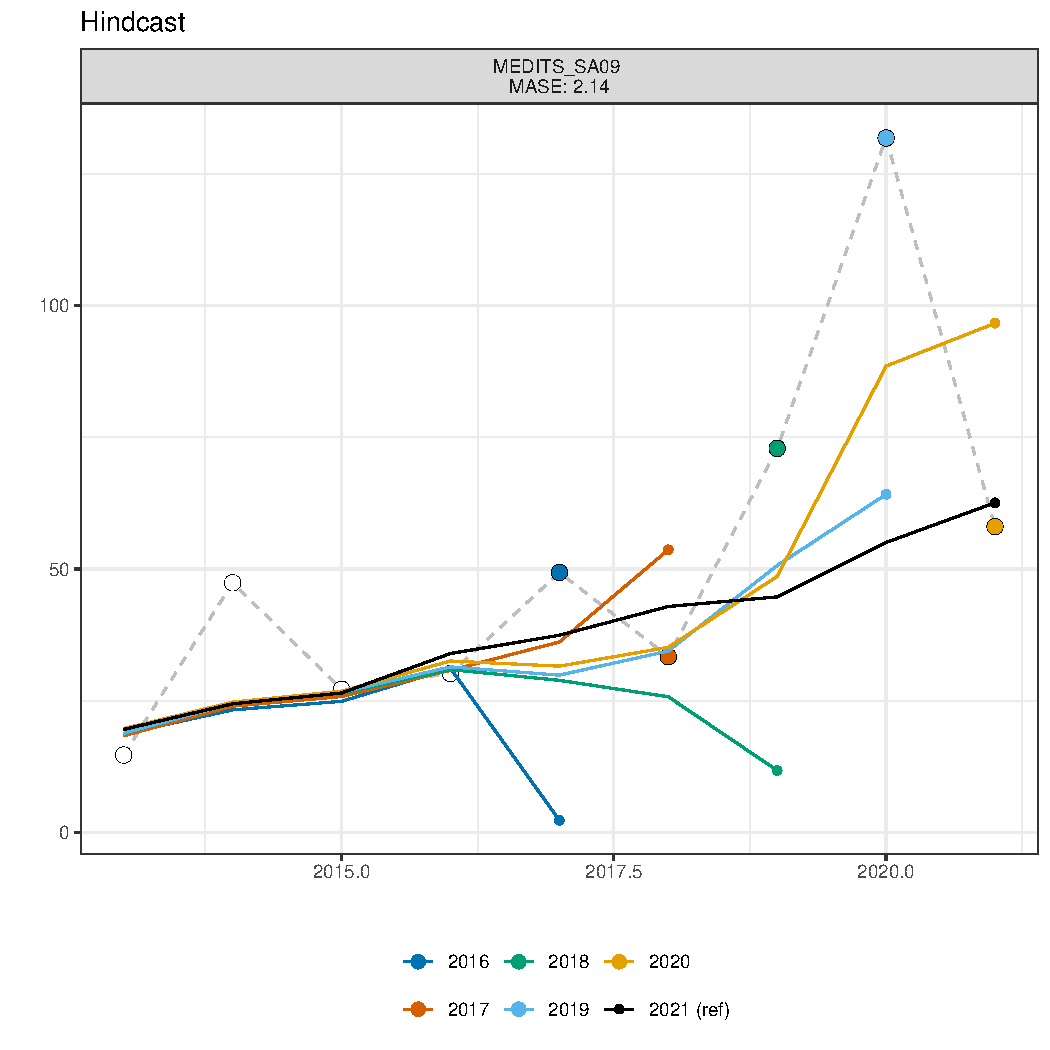
\includegraphics[width=\maxwidth]{figure/xcval-1} \caption[Hindcasting and MASE statistic]{Hindcasting and MASE statistic. A MASE score > 1 indicates that the average model forecasts are worse than a random walk. Conversely, a MASE score of 0.5 indicates that the model forecasts twice as accurately as a naïve baseline prediction; thus, the model has prediction skill}\label{fig:xcval}
\end{figure}

\end{knitrout}


\end{document}
